\section{سوال اول}
در این مسئله تعداد ارسال از تهران به ساری را
$x_1$
و به کاشان را
$x_2$
در نظر می‌گیریم. همچنین،  تعداد ارسال از اصفهان به ساری را
$y_1$
و به کاشان را
$y_2$
در نظر می‌گیریم. تابع هزینه و قیود به صورت زیر در نظر گرفته شده است.
\begin{align*}
	& 5x_1 + 10x_2 + 15y_1 + 4y_2 = \text{cost}  \\
	&x_1 + x_2 \leq 500\\
	&y_1 + y_2 \leq 800\\
	&x_1 + y_1 = 600 \\
	&x_2 + y_2 = 400
\end{align*}
\begin{align*}
	&x_1 + y_1 = 600 \rightarrow y_1 = 600 - x_1\\
	&x_2 + y_2 = 400 \rightarrow y_2 = 400 - x_2\\	
	\rightarrow &y_1 + y_2 \leq 800  \rightarrow 1000 - x_1 -x_2 \leq 800 \rightarrow 200 \leq x_1 + x_2 \leq 500
\end{align*} 
بر اساس قضیه‌ای در \lr{linear programming}
جواب مسئله در مرزهاست و با توجه به تابع هزینه،
$x_1 = 500$
و
$x_2 = 0$
است.
\begin{align*}
	x_1 + y_1 = 600 \xrightarrow{x_1 = 500} y_1 = 100 \\
	x_2 + y_2 = 400 \xrightarrow{x_2 = 0} y_2 = 400
\end{align*}

\begin{figure}[H]
	\caption{محدوده $x_1$ و $x_2$} 
	\centering 
	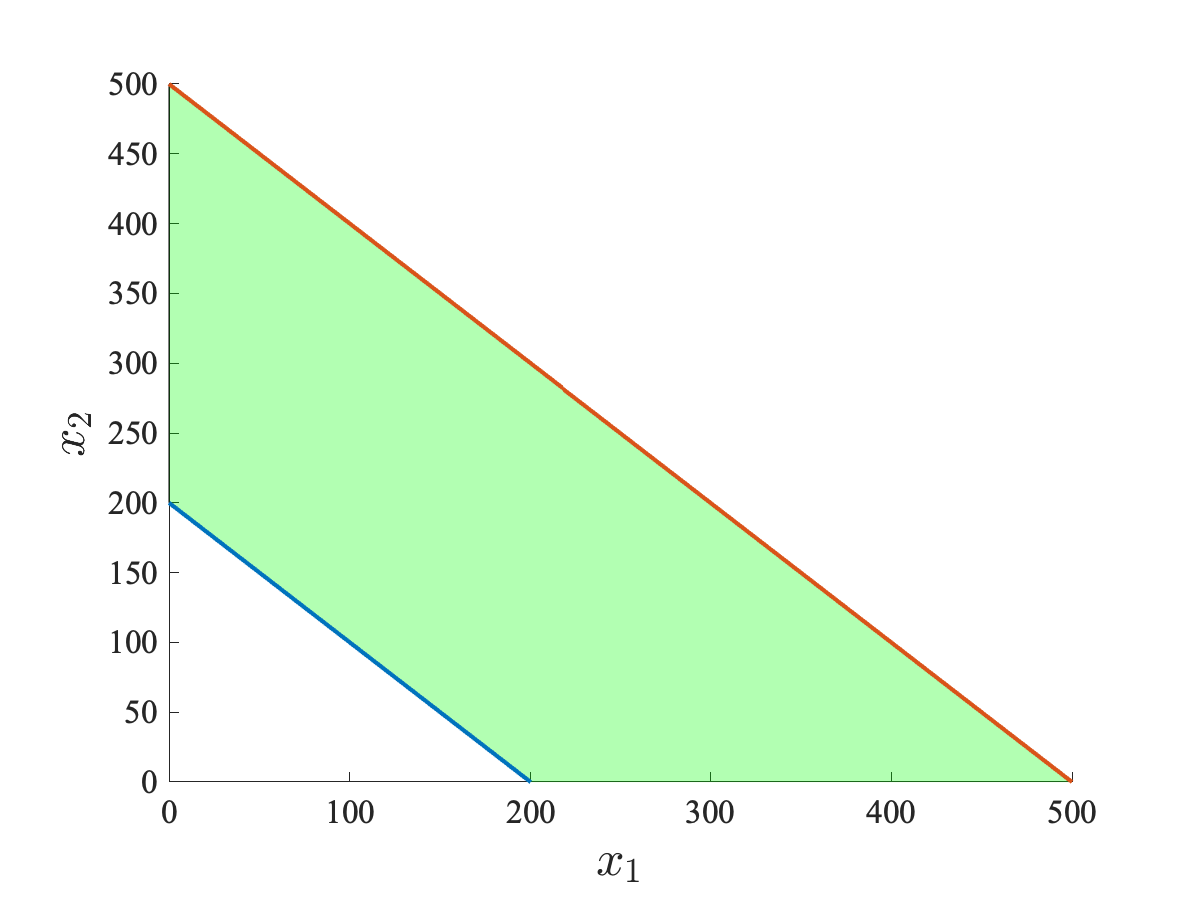
\includegraphics[width=12cm]{../Figure/Q1/valid_x1_x2} 
\end{figure}

\begin{itemize}
	\item ساری
	\begin{align*}
		& 5x_1 + 15y_1 = \text{cost}  \\
		&x_1 + y_1 = 600\\
		&x_1 + x_2 \leq 500\\
		&y_1 + y_2 \leq 800
	\end{align*}
	  \begin{figure}[H]
		\caption{پاسخ گرافیکی شهر ساری} 
		\centering 
		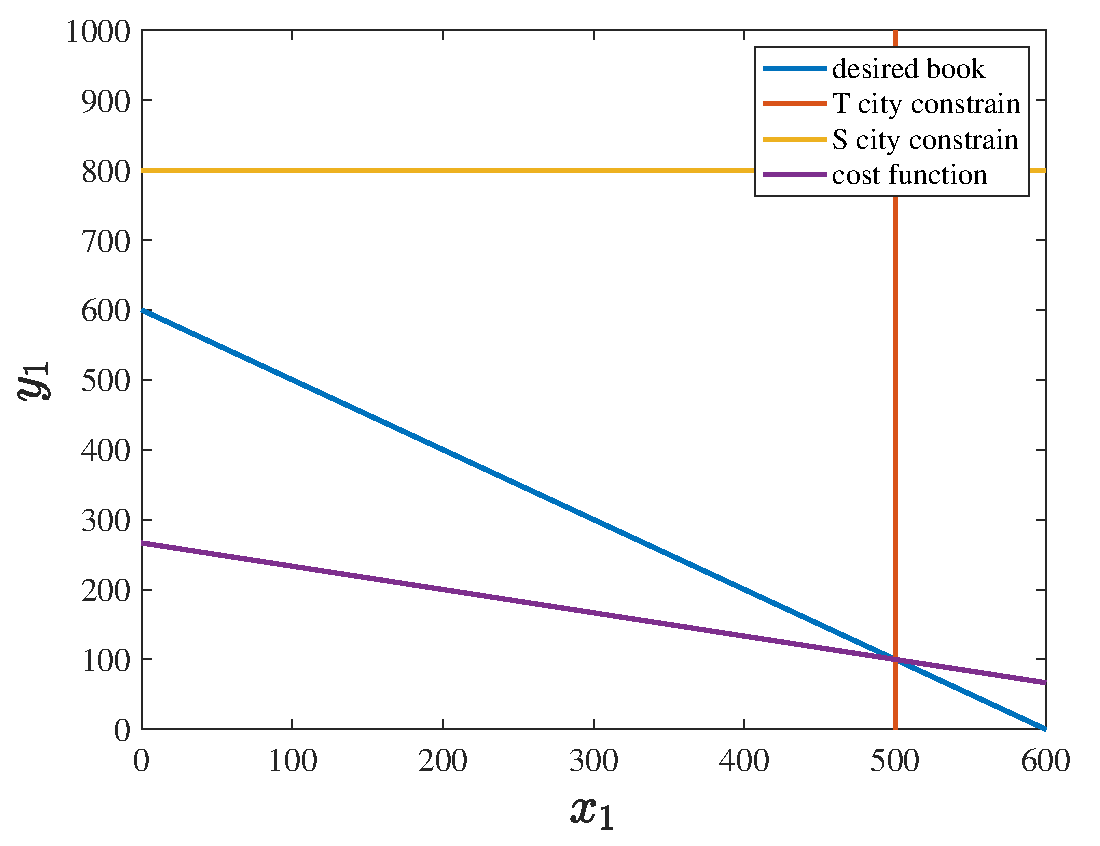
\includegraphics[width=12cm]{../Figure/Q1/S_city} 
	\end{figure}
	\item  کاشان
	\begin{align*}
		& 10x_2 + 4y_2 = \text{cost}  \\
		&x_1 + y_1 = 400\\
		&x_1 + x_2 \leq 500\\
		&y_1 + y_2 \leq 800
	\end{align*}
  \begin{figure}[H]
	\caption{پاسخ گرافیکی شهر کاشان} 
	\centering 
	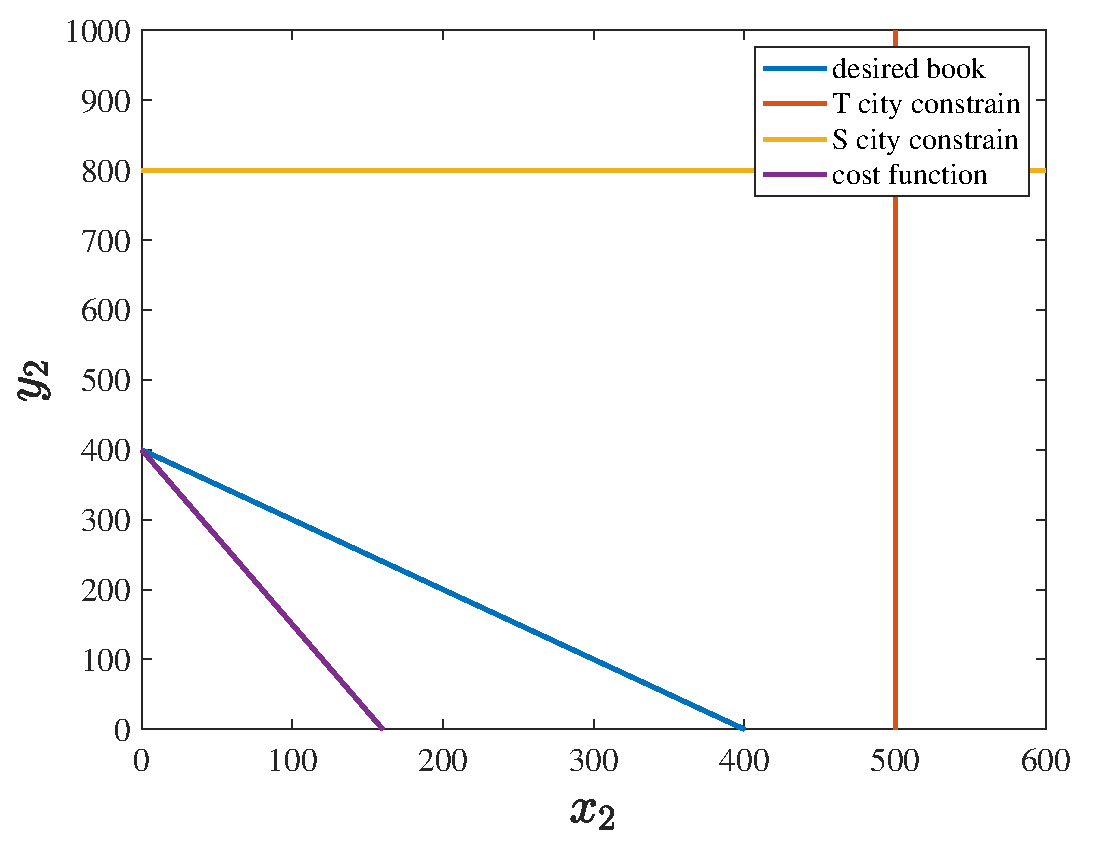
\includegraphics[width=12cm]{../Figure/Q1/K_city} 
\end{figure}
\end{itemize}
در متلب تابعی به نام \lr{linprog}
هست که این مسئله را حل می کند، در پوشه \lr{Q1}
و در فایل \lr{Q1.m}
این مسئله نیز دوباره حل شده است.

